\documentclass[tikz,border=10pt]{standalone}

\usepackage{tikz}
\usetikzlibrary{positioning}
\usetikzlibrary{shapes,arrows,backgrounds,fit,shapes.geometric,calc}
\usetikzlibrary{pgfplots.groupplots}
\usepackage{pgfplots}
\usepackage{pgfplotstable}
\usepackage{listings}
\usepackage{lstautogobble}
\usepackage{color}
\usepackage{bm} % bold math
\usepackage{xspace}

\tikzset{
    %Define standard arrow tip
    >=stealth',
    % Define arrow style
    pil/.style={
           ->,
           thick,
           shorten <=2pt,
           shorten >=2pt,}
}

\newcommand{\vv}[1]{\bm{#1}\xspace}

\begin{document}

%-----------------------------------------------------
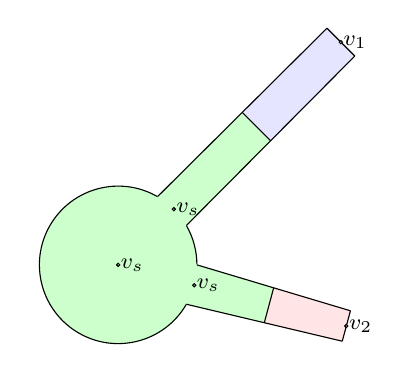
\begin{tikzpicture}[outer sep = 0pt]

%\draw[step=0.5, gray!20, very thin] (-2,-2) grid (4,4);

\coordinate (offset1) at (-0.07071,0.07071);
\coordinate (offset2) at (0.02588,0.09659);

\coordinate (center) at (0,0);

\draw[fill=green!20,green!20](center) circle(1);

\draw        (1,0)    arc (0:30:1)    coordinate(start1a);
\draw[white] (start1a) arc (30:45:1)  coordinate(dend1c);
\draw[white] (dend1c) arc (45:60:1)   coordinate(start1b);

\draw        (start1b) arc (60:330:1) coordinate(start2a);
\draw[white] (start2a) arc (330:345:1) coordinate(dend2c);
\draw[white] (dend2c) arc (345:360:1) coordinate(start2b);

\coordinate (dend1) at ($4*(dend1c)$);
\coordinate (end1a) at ($(dend1) + 2.5*(offset1)$);
\coordinate (end1b) at ($(dend1) - 2.5*(offset1)$);
\coordinate (mid1a) at ($0.5*(end1a) + 0.5*(start1b)$);
\coordinate (mid1b) at ($0.5*(end1b) + 0.5*(start1a)$);
\coordinate (dend2) at ($3*(dend2c)$);
\coordinate (end2a) at ($(dend2) + 2*(offset2)$);
\coordinate (end2b) at ($(dend2) - 2*(offset2)$);
\coordinate (mid2a) at ($0.5*(end2a) + 0.5*(start2b)$);
\coordinate (mid2b) at ($0.5*(end2b) + 0.5*(start2a)$);

\filldraw[fill=green!20,green!20] (start1b) -- (start1a) -- (mid1b) -- (mid1a) -- cycle;
\filldraw[fill=green!20,green!20] (start2b) -- (start2a) -- (mid2b) -- (mid2a) -- cycle;

\filldraw[fill=blue!10,blue!10]   (mid1a) -- (mid1b) -- (end1b) -- (end1a) -- cycle;
\filldraw[fill=red!10,red!10]     (mid2a) -- (mid2b) -- (end2b) -- (end2a) -- cycle;

\draw[fill=white] (0,0)    circle(0.02);
\draw[fill=white] (dend1c) circle(0.02);
\draw[fill=white] (dend2c) circle(0.02);

\draw  (end1a) -- (end1b);
\draw  (start1a) -- (end1b);
\draw  (start1b) -- (end1a);
\draw[fill=white] (dend1) circle(0.02);
\draw (mid1a) -- (mid1b);

\draw  (end2a)   -- (end2b);
\draw  (start2a) -- (end2b);
\draw  (start2b) -- (end2a);
\draw[fill=white] (dend2) circle(0.02);
\draw (mid2a) -- (mid2b);

\node [anchor=west, inner sep=1pt] (mmm) at (center) {\footnotesize $v_{\tiny s}$};
\node [anchor=west, inner sep=1pt] (mmm) at (dend1c) {\footnotesize $v_{\tiny s}$};
\node [anchor=west, inner sep=1pt] (mmm) at (dend2c) {\footnotesize $v_{\tiny s}$};
\node [anchor=west, inner sep=1pt] (mmm) at (dend1) {\footnotesize $v_{\tiny 1}$};
\node [anchor=west, inner sep=1pt] (mmm) at (dend2) {\footnotesize $v_{\tiny 2}$};

\end{tikzpicture}
%-----------------------------------------------------

\end{document}

